\documentclass[twocolumn, 12pt]{article}

\usepackage[utf8]{inputenc}
\usepackage[english, spanish]{babel}
\usepackage{fullpage}
\usepackage{graphicx}
\usepackage{amsmath}
\usepackage{enumitem}
\usepackage{chngcntr}
\usepackage{setspace}
\usepackage{url}
\usepackage{csquotes}
\usepackage{float}
\usepackage{verbatim}
\usepackage{tabularx}
\usepackage{amsmath}
\usepackage{caption}
\usepackage{bm}
\usepackage{colortbl}
\usepackage{xcolor}

\usepackage{multirow}

% \usepackage{hyperref}

\definecolor{LigthGray}{rgb}{0.7098, 0.7294, 0.7215}
\definecolor{LigthGrayPlus}{rgb}{0.6862, 0.7254, 0.7294}
\definecolor{White}{rgb}{1, 1, 1}
\definecolor{Red}{rgb}{1, 0, 0}

\counterwithin{figure}{section}
\renewcommand{\thesection}{\arabic{section}}
\renewcommand{\thesubsection}{\thesection.\arabic{subsection}}
\renewcommand{\baselinestretch}{1.5}

\usepackage[style=apa, maxnames=6, minnames=3, backend=biber]{biblatex}
\DefineBibliographyStrings{english}{%chktex-file 1 chktex-file 6
    andothers = {\em et\addabbrvspace al\adddot}
}
\addbibresource{./Bibliography/bibliography.bib}

\usepackage{array}

\setlength{\parskip}{0pt}

\raggedbottom{}

\newcommand{\bolditalic}[1]{\textbf{\textit{#1}}}

\begin{document}

\begin{titlepage}
    \centering
    
\includegraphics[width=0.3\textwidth]{Images/logo_utb.png}\par\vspace{1cm}
    {\scshape\LARGE Universidad Tecnológica de Bolívar \par}
    \vspace{1cm}

    {\scshape\Large FÍSICA CALOR Y ONDAS \par}
    \vspace{.2cm}

    % chktex-file 8
    {\scshape\Large Grupo 1 \par}
    \vspace{1cm}
    % chktex-file 8
    \slshape {\Large \bfseries{}Informe de Laboratorio No. I\\}
    \slshape {\small \bfseries{} OSCILACIONES MECÁNICAS: MOVIMIENTO ARMÓNICO SIMPLE.}
    \vspace{2cm}

    \slshape {\itshape{} Mauro González, T00067622 \\}
    \slshape {\itshape{} German De Armas Castaño, T00068765 \\}
    \slshape {\itshape{} Angel Vega Rodriguez, T00068186 \\}
    \slshape {\itshape{} Juan Jose Osorio Ariza, T00067316 \\}
    \slshape {\itshape{} Jorge Alberto Rueda Salgado, T00068722 \\}
    \vfill
    Revisado Por \\
    Duban Andres Paternina Verona\\
    {\large \today\par}
\end{titlepage}

% ! ----------------------------------------------------------------------|>
\section{Introducción}

Las oscilaciones mecánicas constituyen un fenómeno
fundamental en el estudio de la física, abarcando una
amplia variedad de sistemas, desde partículas microscópicas
hasta estructuras macroscópicas. Un ejemplo destacado de
estas oscilaciones es el movimiento armónico simple, en el
que un sistema realiza un vaivén periódico alrededor de una
posición de equilibrio. Este tipo de movimiento presenta
características intrínsecas que permiten su análisis y
comprensión a través de la aplicación de leyes y fórmulas
específicas.

\vspace{.5cm}

En esta experiencia de laboratorio, nos centraremos en la
exploración y comprobación de los conceptos relacionados
con el movimiento armónico simple y su aplicación en la
determinación experimental del período de oscilación de
diferentes tipos de péndulos. Para ello, utilizaremos una
variedad de equipos y simuladores que nos permitirán
observar y analizar las propiedades fundamentales de los
sistemas oscilatorios y su relación con las leyes físicas
que los rigen.

% ! ----------------------------------------------------------------------|>
\section{Objetivos}

% + ----------------------------------------|>
\subsection{Objetivo general}

\begin{itemize}[label=$\triangleright$]
    \item Comprobar experimentalmente la validez de las fórmulas
          utilizadas para calcular el período de oscilación de
          péndulos simples y compuestos, a través de la aplicación de
          principios del movimiento armónico simple.
\end{itemize}

% + ----------------------------------------|>
\subsection{Objetivos específicos}

\begin{itemize}[label=$\triangleright$]
    \item Familiarizarse con los conceptos de oscilación y movimiento
          armónico simple mediante el estudio y análisis previo de
          las propiedades de los sistemas oscilatorios.

    \item Identificar las características clave de un movimiento
          armónico simple, tales como amplitud, período, frecuencia,
          frecuencia angular y fase inicial, y comprender su
          significado físico.

    \item Comprender y aplicar las fórmulas que permiten calcular el
          período de oscilación para distintos tipos de péndulos,
          incluyendo el péndulo simple, el péndulo de resorte y el
          péndulo compuesto.
\end{itemize}

% ! ----------------------------------------------------------------------|>
\section{Marco Teórico}

% + ----------------------------------------|>
\subsection{Oscilaciones armónicas}

Estas son las características Fundamentales de las
Oscilaciones y Péndulos:

\begin{itemize}[label=$\triangleright$]
    \item Amplitud [{\large $A$}]: Elongación máxima. Su unidad de
          medidas en el Sistema Internacional es el metro
          \bolditalic{(m)}.

    \item Periodo [{\large $T$}]: El tiempo que tarda en cumplirse
          una oscilación completa. Es la inversa de la frecuencia $T
              = \frac{1}{f}$. Su unidad de medida en el Sistema
          Internacional es el segundo \bolditalic{(s)}.

    \item Frecuencia [{\large $f$}]: El número de oscilaciones o
          vibraciones que se producen en un segundo. Su unidad de
          medida en el Sistema Internacional es el Hercio (Hz). 1 Hz
          = 1 oscilación / segundo = $1 s^{-1}$.

    \item Frecuencia angular [{\large $\omega$}]: Representa la
          velocidad de cambio de la fase del movimiento. Se trata del
          número de periodos comprendidos en $2\pi$ segundos. Su
          unidad de medida en el sistema internacional es el radián
          por segundo (\@~rad/s\@~). Su relación con el período y la
          frecuencia es: {\large
          \begin{equation}
              \omega = \frac{2 \cdot \pi}{T} = 2 \cdot \pi f
          \end{equation}
          }

    \item Fase [{\large $\phi$}]: Se trata del ángulo que representa
          el estado inicial de vibración, es decir, la elongación x
          del cuerpo en el instante t = 0. Su unidad de medida en el
          Sistema Internacional es el radián (rad).
\end{itemize}

\nocite{movimiento-armonico-simple}

% + ----------------------------------------|>
\subsection{Péndulo simple}

El periodo de un péndulo simple depende de su longitud y de
la aceleración debido a la gravedad. El periodo es
completamente independiente de otros factores, como masa y
desplazamiento máximo.

{\large
\begin{equation}
    T = 2\pi \cdot \sqrt{\frac{L}{g}}
    \label{eq:periodo_pendulo_simple}
\end{equation}
}

\nocite{tipos-pendulos-1}

% + ----------------------------------------|>
\subsection{Péndulo compuesto o físico}

En el caso del péndulo físico, la fuerza gravitatoria
ejerce influencia sobre el centro de masa (CM) del objeto.
Cuando un péndulo físico está suspendido de un punto,
permitiendo su movimiento rotativo, este ocurre debido al
torque aplicado en el CM\@. Este torque es originado por la
componente del peso del objeto que actúa tangencialmente a
la dirección del movimiento del CM\@.

{\large
\begin{equation}
    T = 2\pi \cdot \sqrt{\frac{I}{m g L}}
    \label{eq:periodo_pendulo_fisico}
\end{equation}
}

\nocite{tipos-pendulos-1}

% + ----------------------------------------|>
\subsection{Péndulo de resorte}

El período de un péndulo de resorte se refiere al tiempo
que le toma a una masa conectada a un resorte completar un
ciclo completo de oscilación, yendo desde una posición
extrema a la otra y regresando.

    {\large
        \begin{equation}
            T = 2\pi \cdot \sqrt{\frac{m}{k}}
            \label{eq:periodo_pendulo_resorte}
        \end{equation}
    }

\nocite{tipos-pendulos-2}

% ! ----------------------------------------------------------------------|>
\section{Montaje Experimental}

\begin{figure}[H]
    \begin{center}
        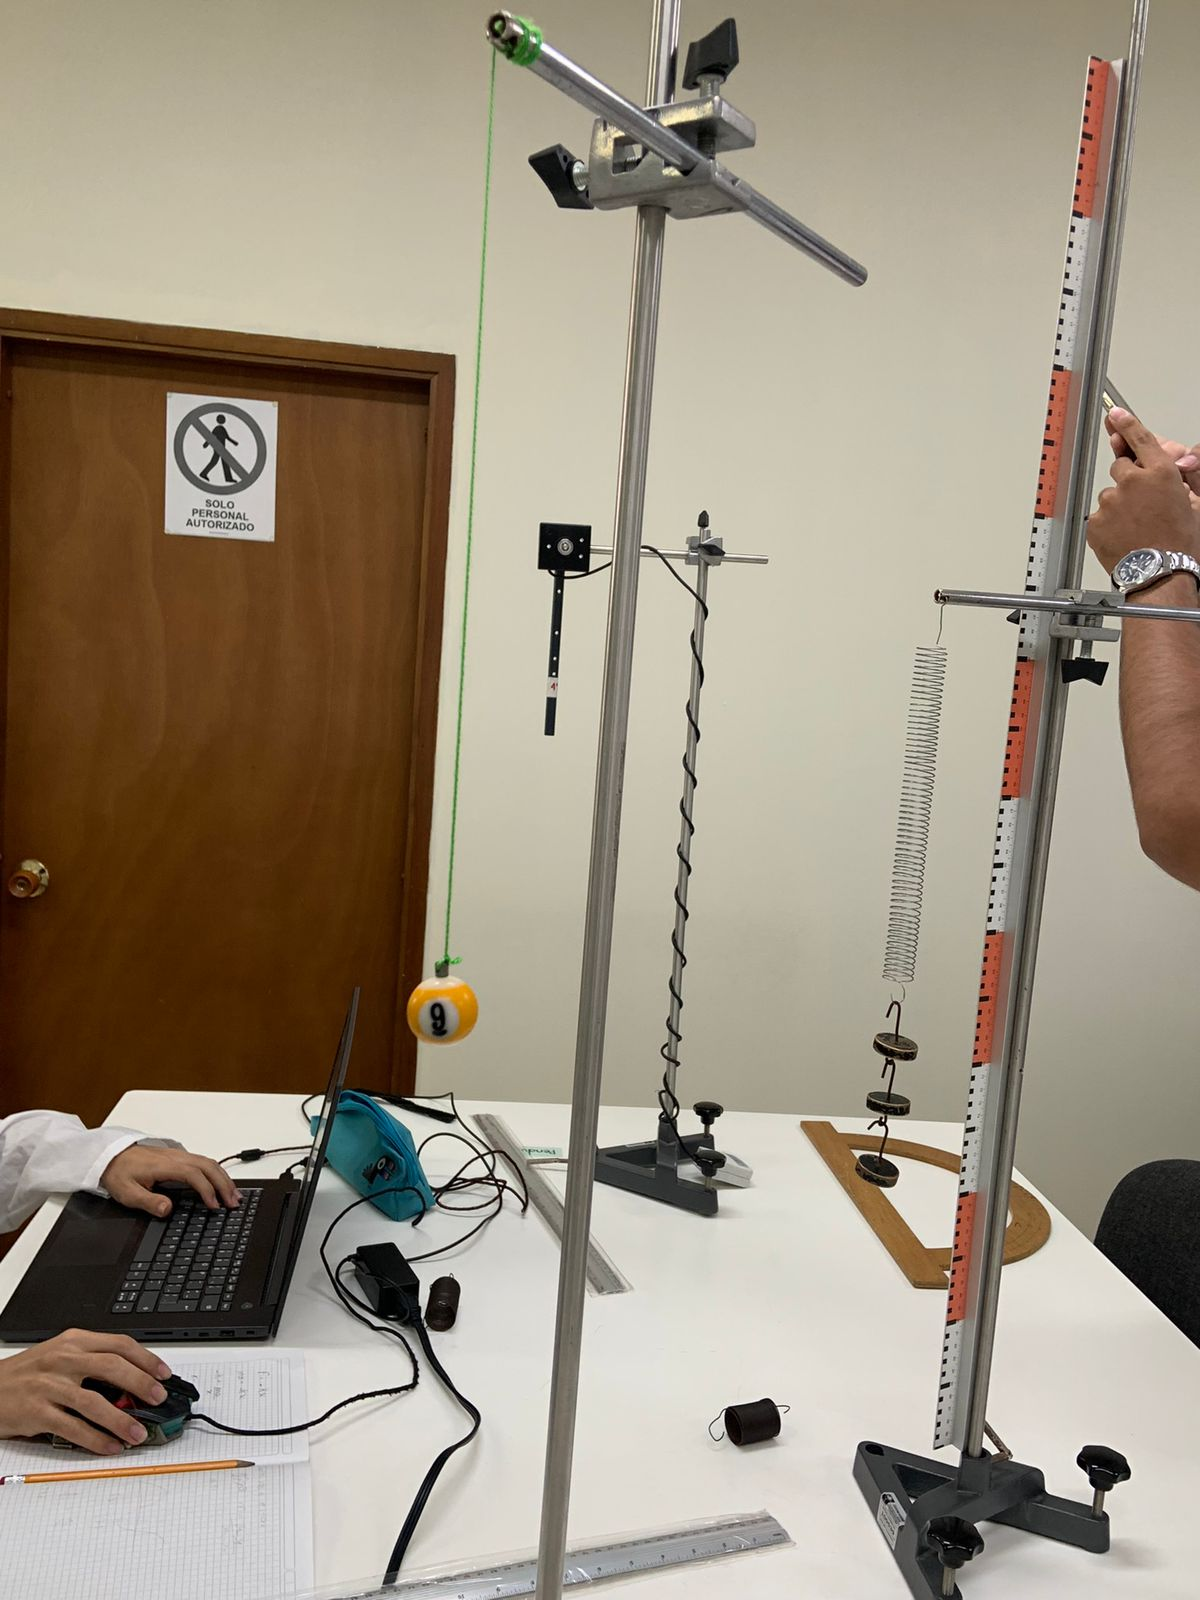
\includegraphics[width=0.6\linewidth]{./Images/IMAGEN_1.jpeg}
    \end{center}
    \caption{Péndulo simple}
\end{figure}

\begin{figure}[H]
    \begin{center}
        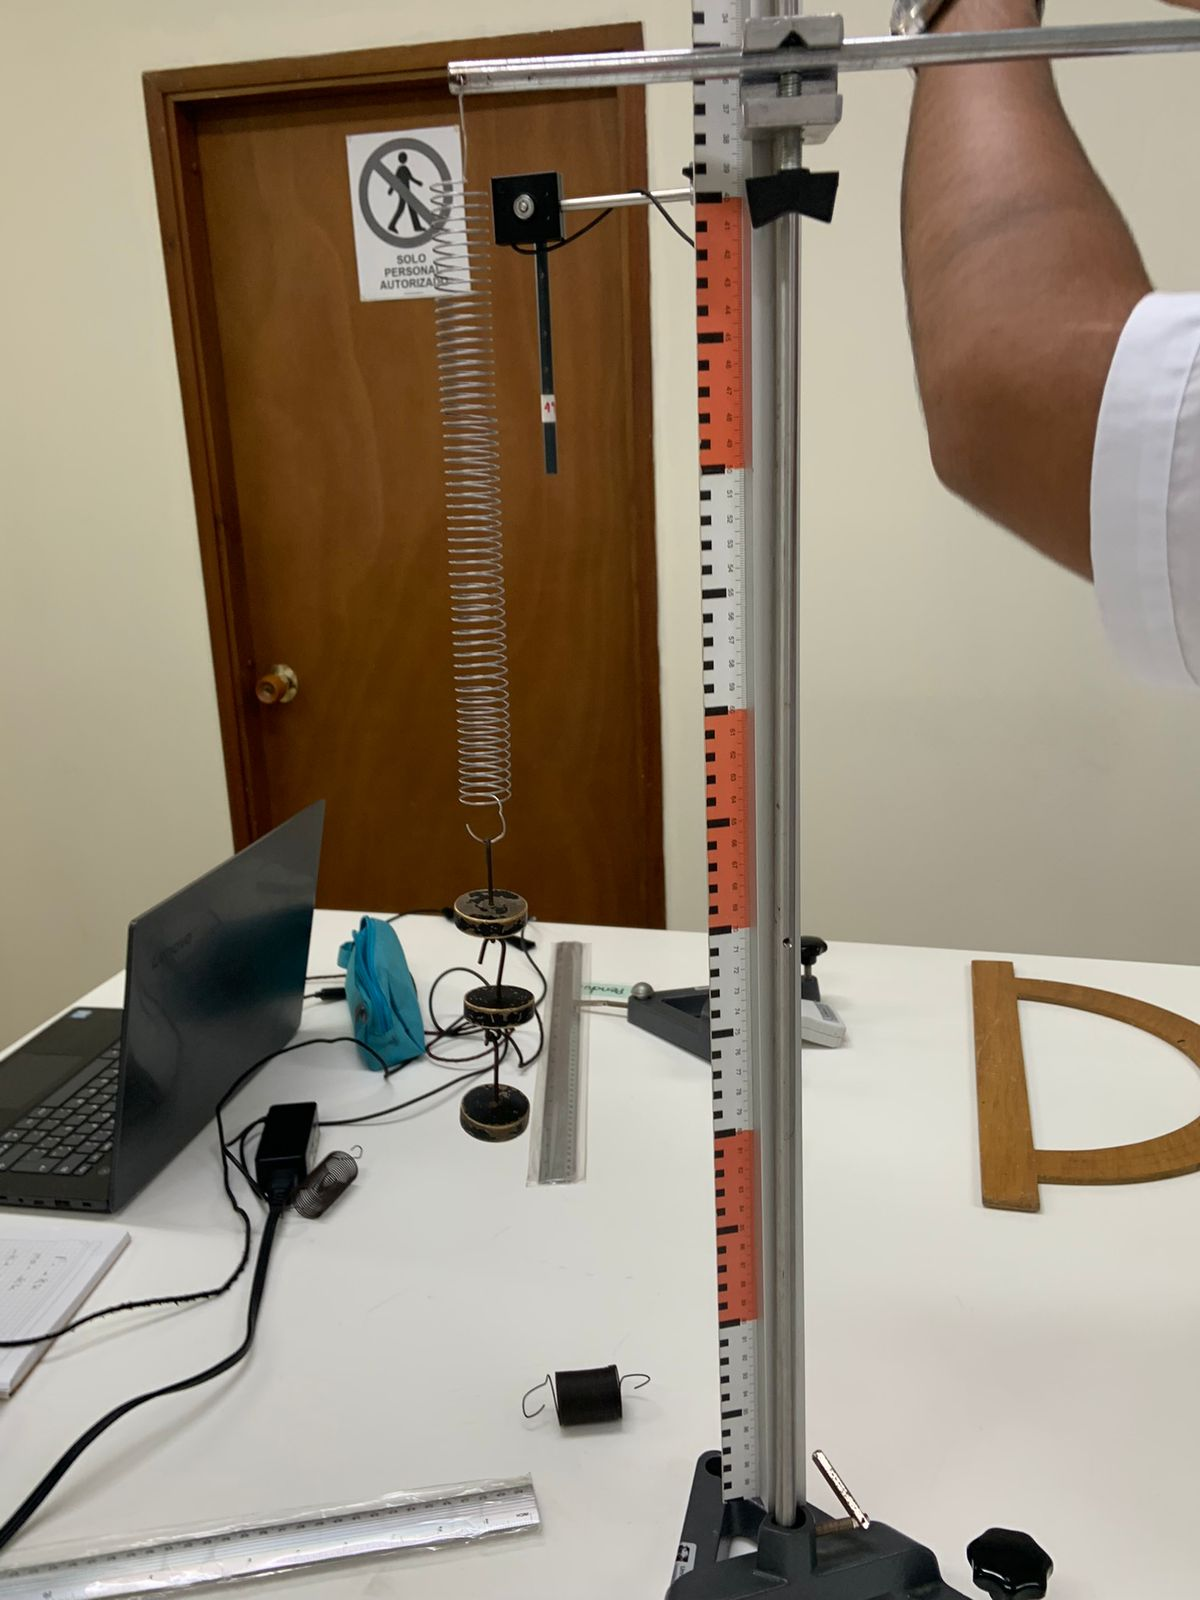
\includegraphics[width=0.6\linewidth]{./Images/IMAGEN_2.jpeg}
    \end{center}
    \caption{Péndulo de resorte}
\end{figure}

\begin{figure}[H]
    \begin{center}
        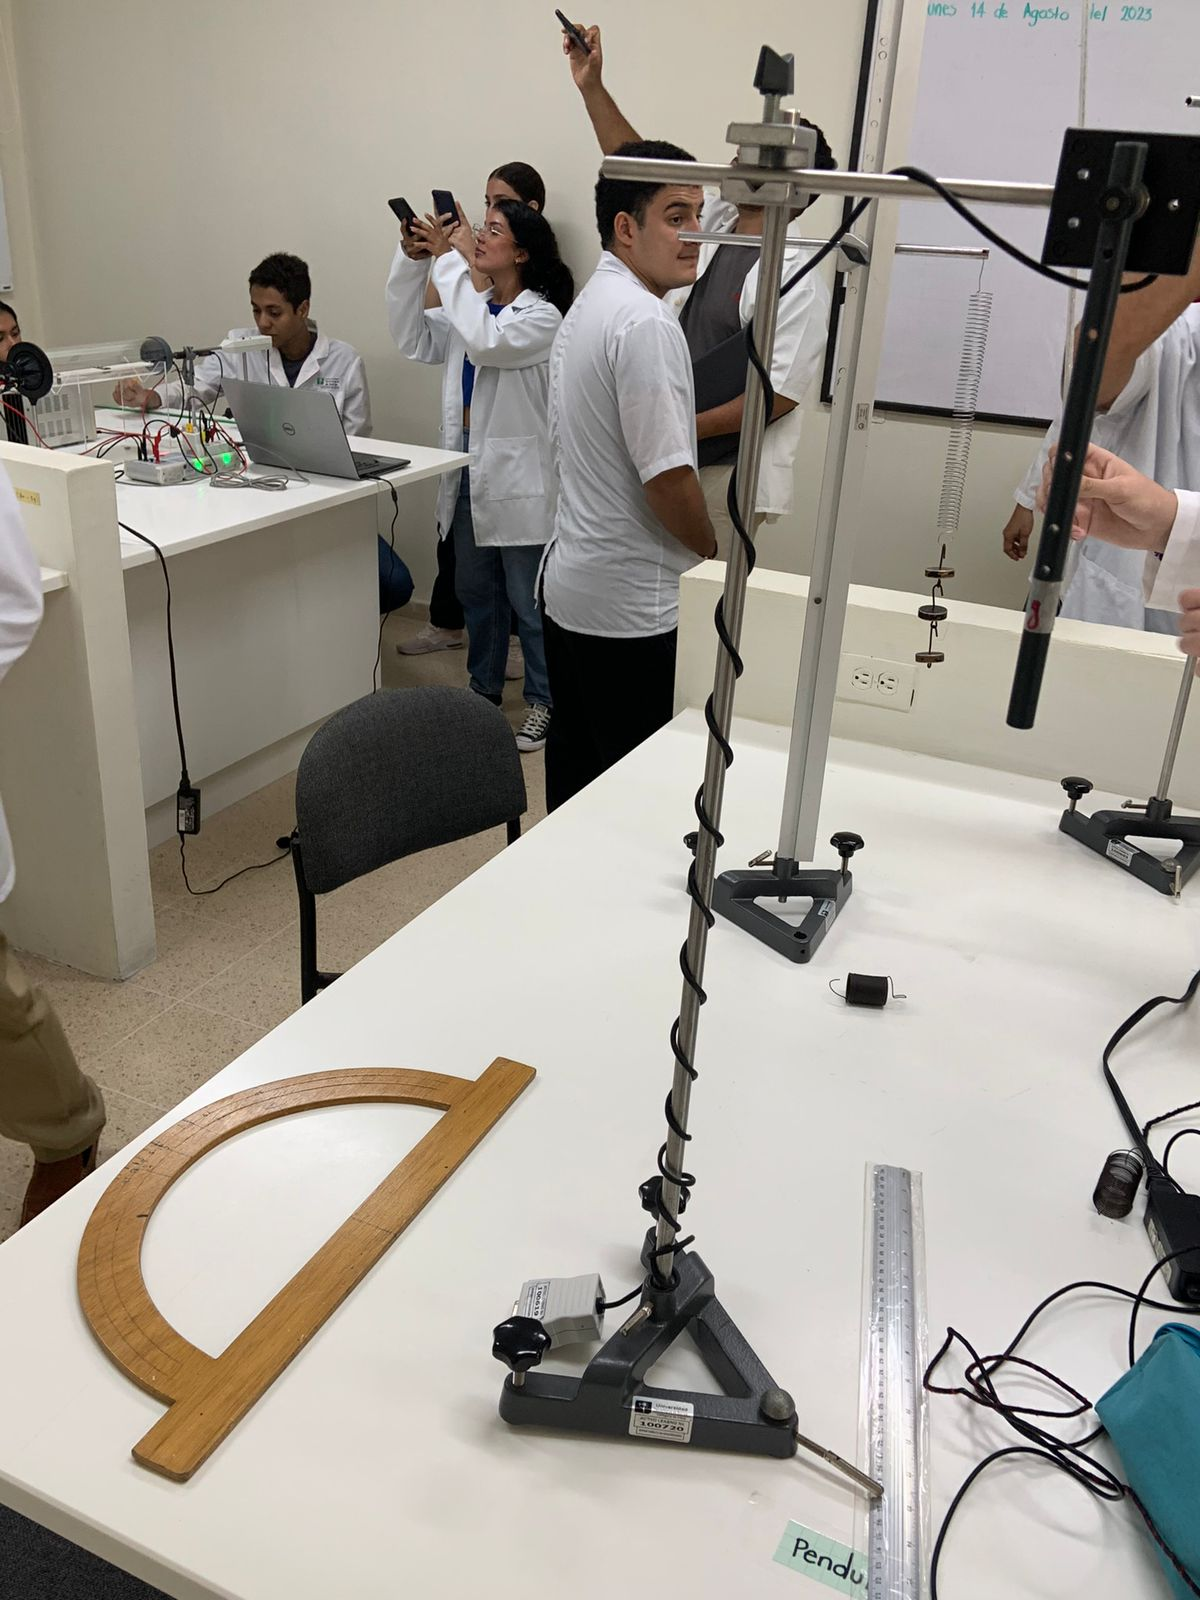
\includegraphics[width=0.6\linewidth]{./Images/IMAGEN_3.jpeg}
    \end{center}
    \caption{Péndulo compuesto}
\end{figure}

\begin{table}[H]
    % chktex-file 44
    \begin{tabularx}{\linewidth}{|>{\centering\arraybackslash}X|>{\centering\arraybackslash}X|>{\centering\arraybackslash}X|}
        \hline
        \rowcolor{LigthGray} Magnitud                     & Símbolo & Unidad                                   \\\hline
        Periodo                                           & T       & Segundos \bolditalic{(s)}                \\\hline
        \rowcolor{LigthGrayPlus} Masa                     & m       & Kilogramos (Kg)                          \\\hline
        Longitud                                          & m       & Metros (m)                               \\\hline
        \rowcolor{LigthGrayPlus} Constante de elasticidad & K       & Newton / Metro (N/m)                     \\\hline
        Gravedad                                          & g       & Metros / Segundo al cuadrado $(m/s^{2})$ \\\hline
    \end{tabularx}
\end{table}

% ! ----------------------------------------------------------------------|>
\section{Datos Experimentales}

% + ----------------------------------------|>
\subsection{Péndulo Simple}

% chktex-file 44

\begin{table}[H]
    \begin{tabularx}{\linewidth}{|>{\centering\arraybackslash}X|>{\centering\arraybackslash}X|>{\centering\arraybackslash}X|}
        \hline
        \rowcolor{LigthGray} No.   & Longitud \bolditalic{(M)} & Angulo \bolditalic{(°)} \\ \hline
        1                          & 0.3700                    & 15.0000                 \\\hline
        \rowcolor{LigthGrayPlus} 2 & 0.3050                    & 15.0000                 \\\hline
        3                          & 0.4450                    & 15.0000                 \\\hline
    \end{tabularx}

\end{table}

\vspace{-.5cm}

\begin{table}[H]
    \begin{tabularx}{\linewidth}{|>{\centering\arraybackslash}X|>{\centering\arraybackslash}X|>{\centering\arraybackslash}X|}
        \hline
        \rowcolor{LigthGray} \multicolumn{3}{|c|}{Tiempo \bolditalic{(s)}} \\ \hline
        12.4100                          & 12.5100 & 12.1100               \\ \hline
        \rowcolor{LigthGrayPlus} 11.7000 & 11.1500 & 11.0300               \\\hline
        13.5000                          & 13.2800 & 13.3800               \\\hline
    \end{tabularx}

\end{table}

\vspace{-.5cm}

\begin{table}[H]
    \begin{tabularx}{\linewidth}{|>{\centering\arraybackslash}X|>{\centering\arraybackslash}X|}
        \hline
        \rowcolor{LigthGray} Promedio \bolditalic{(s)} & Periodo \bolditalic{(S)} \\ \hline
        12.3433                                        & 1.2343                   \\\hline
        \rowcolor{LigthGrayPlus} 11.2933               & 1.1293                   \\\hline
        13.3867                                        & 1.3387                   \\\hline
    \end{tabularx}

\end{table}

\vspace{-.5cm}

\begin{table}[H]
    \begin{tabularx}{\linewidth}{|>{\centering\arraybackslash}X|>{\centering\arraybackslash}X|}
        \hline
        \rowcolor{LigthGrayPlus} \textbf{Oscilaciones} & 10 \\\hline
    \end{tabularx}
\end{table}

% + ----------------------------------------|>
\subsection{Péndulo Compuesto}

\begin{table}[H]
    \begin{tabularx}{\linewidth}{|>{\centering\arraybackslash}X|>{\centering\arraybackslash}X|>{\centering\arraybackslash}X|>{\centering\arraybackslash}X|}
        \hline
        \rowcolor{LigthGray} No. & Masa \bolditalic{(Kg)} & Longitud \bolditalic{(M)} & Distancia \bolditalic{(M)} \\ \hline
        1                        & 0,0490                 & \multirow{3}{*}{0.2470}   & 0,0500                     \\
        2                        & 0,0490                 &                           & 0,0840                     \\
        3                        & 0,0490                 &                           & 0,1020                     \\\hline
    \end{tabularx}
\end{table}

\vspace{-.5cm}

\begin{table}[H]
    \begin{tabularx}{\linewidth}{|>{\centering\arraybackslash}X|>{\centering\arraybackslash}X|>{\centering\arraybackslash}X|}
        \hline
        \rowcolor{LigthGray} \multicolumn{3}{|c|}{Tiempo \bolditalic{(s)}} \\ \hline
        4,0000                          & 3,7100 & 3,7400                  \\\hline
        \rowcolor{LigthGrayPlus} 3,8400 & 3,7000 & 4,1000                  \\\hline
        3,9000                          & 3,8100 & 3,9800                  \\\hline

    \end{tabularx}
\end{table}

\vspace{-.5cm}

\begin{table}[H]
    \begin{tabularx}{\linewidth}{|>{\centering\arraybackslash}X|>{\centering\arraybackslash}X|}
        \hline
        \rowcolor{LigthGray} Promedio \bolditalic{(s)} & Periodo \bolditalic{(S)} \\ \hline
        3,8167                                         & 0,7633                   \\\hline
        \rowcolor{LigthGrayPlus} 3,8800                & 0,7760                   \\\hline
        3,8967                                         & 0,7793                   \\\hline
    \end{tabularx}
\end{table}

\vspace{-.5cm}

\begin{table}[H]
    \begin{tabularx}{\linewidth}{|>{\centering\arraybackslash}X|>{\centering\arraybackslash}X|}
        \hline
        \rowcolor{LigthGrayPlus} \textbf{Oscilaciones} & 5 \\\hline
    \end{tabularx}
\end{table}

% + ----------------------------------------|>
\subsection{Péndulo de Resorte}

\begin{table}[H]
    \begin{tabularx}{\linewidth}{|>{\centering\arraybackslash}X|>{\centering\arraybackslash}X|}
        \hline
        \rowcolor{LigthGray} No.   & Masa \bolditalic{(Kg)} \\\hline
        1                          & 0,0100                 \\\hline
        \rowcolor{LigthGrayPlus} 2 & 0,0150                 \\\hline
        3                          & 0,0200                 \\\hline
    \end{tabularx}
\end{table}

\vspace{-.5cm}

\begin{table}[H]
    \begin{tabularx}{\linewidth}{|>{\centering\arraybackslash}X|>{\centering\arraybackslash}X|}
        \hline
        \rowcolor{LigthGray} Longitud Inicial \bolditalic{(M)} & Longitud Final \bolditalic{(M)} \\\hline
        1                                                      & 0,0100                          \\\hline
        \rowcolor{LigthGrayPlus} 2                             & 0,0150                          \\\hline
        3                                                      & 0,0200                          \\\hline
    \end{tabularx}
\end{table}

\vspace{-.5cm}

\begin{table}[H]
    \begin{tabularx}{\linewidth}{|>{\centering\arraybackslash}X|>{\centering\arraybackslash}X|}
        \hline
        \rowcolor{LigthGray} $\Delta X$ \bolditalic{(M)} & K \bolditalic{(N/m)} \\\hline
        0,0750                                           & 1,3080               \\\hline
        0,1100                                           & 1,3377               \\\hline
        0,1500                                           & 1,3080               \\\hline
    \end{tabularx}
\end{table}

\vspace{-.2cm}

\begin{itemize}[label=$\triangleright$]
    \item K Promedio:~\textcolor{Red}{$1.3179$}
\end{itemize}

\vspace{-.2cm}

\begin{table}[H]
    \begin{tabularx}{\linewidth}{|>{\centering\arraybackslash}X|>{\centering\arraybackslash}X|>{\centering\arraybackslash}X|}
        \hline
        \rowcolor{LigthGray} \multicolumn{3}{|c|}{Tiempo \bolditalic{(s)}} \\ \hline
        5,5400                          & 5,5300 & 5,1700                  \\\hline
        \rowcolor{LigthGrayPlus} 6,1300 & 6,2000 & 6,3600                  \\\hline
        8,1300                          & 7,2600 & 7,9600                  \\\hline
    \end{tabularx}
\end{table}

\vspace{-.5cm}

\begin{table}[H]
    \begin{tabularx}{\linewidth}{|>{\centering\arraybackslash}X|}
        \hline
        \rowcolor{LigthGray} Promedio \bolditalic{(s)} \\ \hline
        5,4133                                         \\\hline
        \rowcolor{LigthGrayPlus} 6,2300                \\\hline
        7,7833                                         \\\hline

    \end{tabularx}
\end{table}

\vspace{-.5cm}

\begin{table}[H]
    \begin{tabularx}{\linewidth}{|>{\centering\arraybackslash}X|>{\centering\arraybackslash}X|}
        \hline
        \rowcolor{LigthGrayPlus} \textbf{Oscilaciones} & 10 \\\hline
    \end{tabularx}
\end{table}

% ! ----------------------------------------------------------------------|>
\section{Análisis de datos}

% + ----------------------------------------|>
\subsection{Comprobación experimental}

Usando la formula,

\begin{equation}
    \frac{\left\lvert Teorico - Experimental\right\rvert }{Teorico} \times 100
\end{equation}

\begin{table}[H]
    \begin{tabularx}{\linewidth}{|>{\centering\arraybackslash}X|>{\centering\arraybackslash}X|>{\centering\arraybackslash}X|>{\centering\arraybackslash}X|}
        \multicolumn{4}{c}{Pendulo simple Teorico vs Experimental}               \\\hline
        \rowcolor{LigthGray} \multicolumn{4}{|c|}{\bolditalic{Periodo}}          \\\hline

                                                      & 1      & 2      & 3      \\ \hline
        \rowcolor{LigthGrayPlus} \textbf{Teórico}     & 1.2208 & 1.1084 & 1.3389 \\\hline
        \textbf{Experi-\newline{}mental}              & 1,243  & 1,1293 & 1,3387 \\\hline
        \rowcolor{LigthGrayPlus} \textbf{\% de error} & 1,8185 & 1,8856 & 0,0149 \\\hline
    \end{tabularx}
    % chktex-file 24
    \caption{}
    \label{tab:comprobacion_pendulo_simple}
\end{table}

\begin{table}[H]
    \begin{tabularx}{\linewidth}{|>{\centering\arraybackslash}X|>{\centering\arraybackslash}X|>{\centering\arraybackslash}X|>{\centering\arraybackslash}X|}
        \multicolumn{4}{c}{Pendulo fisico Teorico vs Experimental}               \\\hline
        \rowcolor{LigthGray} \multicolumn{4}{|c|}{\bolditalic{Periodo}}          \\\hline

                                                      & 1      & 2      & 3      \\ \hline
        \rowcolor{LigthGrayPlus} \textbf{Teórico}     & 0,7817 & 0,763  & 0,7821 \\\hline
        \textbf{Experi-\newline{}mental}              & 0,7633 & 0,776  & 0,7793 \\\hline
        \rowcolor{LigthGrayPlus} \textbf{\% de error} & 2,3538 & 1,7038 & 0,3580 \\\hline
    \end{tabularx}
    \caption{}
    \label{tab:comprobacion_pendulo_fisico}
\end{table}

\begin{table}[H]
    \begin{tabularx}{\linewidth}{|>{\centering\arraybackslash}X|>{\centering\arraybackslash}X|>{\centering\arraybackslash}X|>{\centering\arraybackslash}X|}
        \multicolumn{4}{c}{Pendulo resorte Teorico vs Experimental}              \\\hline
        \rowcolor{LigthGray} \multicolumn{4}{|c|}{\bolditalic{Periodo}}          \\\hline

                                                      & 1      & 2      & 3      \\ \hline
        \rowcolor{LigthGrayPlus} \textbf{Teórico}     & 0,5494 & 0,6728 & 0,7769 \\\hline
        \textbf{Experi-\newline{}mental}              & 0,5413 & 0,623  & 0,7783 \\\hline
        \rowcolor{LigthGrayPlus} \textbf{\% de error} & 1,4743 & 7,4019 & 0,1802 \\\hline
    \end{tabularx}
    \caption{}
    \label{tab:comprobacion_pendulo_resorte}
\end{table}

% + ----------------------------------------|>
\subsection{Análisis}

En esta primera práctica, se llevó a cabo la recolección de
datos relacionados con todas las variables que influyen en
el periodo de oscilación en diferentes tipos de péndulos.
Estos datos fueron recopilados con el propósito de comparar
posteriormente los resultados experimentales con sus
valores teóricos.

% + ----------------------------------------|>
\subsubsection{}

Sí, esta situación es claramente demostrada en las tablas
(\ref{tab:comprobacion_pendulo_simple},~\ref{tab:comprobacion_pendulo_fisico},~\ref{tab:comprobacion_pendulo_resorte}),
y esto ocurre debido a que estas fórmulas se basan en
situaciones ideales, considerando las características
físicas específicas de cada tipo de péndulo. En el caso del
péndulo simple, su periodo se ve influenciado por la
longitud de la cuerda. En cuanto al péndulo de resorte, son
la constante de elasticidad y la masa los factores que
afectan su periodo, mientras que, en el caso de un péndulo
físico, los determinantes son el momento de inercia y la
longitud de la cuerda.

% + ----------------------------------------|>
\subsubsection{}

Esto se debe al margen de error que se ha presentado al
registrar los diferentes intervalos de tiempo, influencias
de medición inexacta y factores derivados de la interacción
humana, además de elementos del entorno externo como la
resistencia del aire.

% + ----------------------------------------|>
\subsubsection{}

\begin{itemize}[label=$\triangleright$]
    \item Péndulo simple \\ Despejando la
          ecuación~(\ref{eq:periodo_pendulo_simple}), donde $T = 1s$
          y $g = 9.8 \frac{m}{s^{2}}$

          \begin{equation*}
              \begin{gathered}
                  1s = 2 \pi \sqrt{\frac{L}{9.8 \frac{m}{s^{2}}}} \\
                  \frac{1s}{2 \pi} =  \sqrt{\frac{L}{9.8 \frac{m}{s^{2}}}} \\
                  {(\frac{1s}{2 \pi})}^{2} =  \frac{L}{9.8 \frac{m}{s^{2}}} \\
                  {(0.1591)}^{2} = \frac{L}{9.8 \frac{m}{s^{2}}} \\
                  (0.025) \cdot (9.8 \frac{m}{s^{2}}) = L \\
                  L = 0.2482 m
              \end{gathered}
          \end{equation*}

    \item Péndulo físico \\ Despejando la
          ecuación~(\ref{eq:periodo_pendulo_fisico}), donde $T = 1s$
          y $I = \frac{1}{3} m L^{2}$
          \begin{equation*}
              \begin{gathered}
                  1s = 2 \pi \sqrt{\frac{I}{m g d}} \\
                  T = 2 \pi \sqrt{\frac{\frac{1}{3} m L^{2}}{m g d}} \\
                  T = 2 \pi \sqrt{\frac{\frac{1}{3} L^{2}}{g \frac{L}{2}}} \\
                  T = 2 \pi \sqrt{\frac{2L}{3g}} \\
                  T^{2} = 4\pi^{2} \cdot \frac{2L}{3g} \\
                  {(1s)}^{2} = (39.5) \cdot (\frac{2L}{3 (9.81 \frac{m}{s^{2}})})\\
                  L = \frac{{(1s)}^{2} \cdot (\frac{29.43m}{s^{2}})}{78.4}\\
                  L = 0.375m
              \end{gathered}
          \end{equation*}
    \item Péndulo de resorte \\ Despejando la
          ecuación~(\ref{eq:periodo_pendulo_resorte})
          \begin{equation*}
              \begin{gathered}
                  \frac{T}{2\pi} = \sqrt{\frac{m}{K}} \\
                  \frac{T^2}{4 \pi^2} = \frac{m}{K} \\
                  K = 4 \pi^2 m \\
                  \frac{m a}{x} = 4 \pi^2 m \\
                  \frac{g}{x} = 4 \pi^2 \\
                  x = \frac{4\pi^2}{g}\\
                  x = 4.024 cm = 0.04 m
              \end{gathered}
          \end{equation*}
\end{itemize}

% ! ----------------------------------------------------------------------|>
\section{Conclusiones}

A lo largo del informe titulado ``Oscilaciones mecánicas:
Movimiento armónico simple'', se llevó a cabo un análisis
experimental con el objetivo de determinar, comprender y
explicar las características del periodo de oscilación en
varios tipos de péndulos.

Durante el desarrollo del informe, se observó la relación
entre las variables que interactúan en el periodo de
oscilación. En el caso del péndulo simple, se pudo observar
que el período de oscilación es independiente de la
amplitud y la masa del objeto. Esto se alinea con la teoría
del movimiento armónico simple, la cual establece que el
período solo depende de la longitud del péndulo y la
aceleración debida a la gravedad.

Al analizar un péndulo físico (un objeto con dimensiones
físicas apreciables), se encontró que su período de
oscilación no depende únicamente de la longitud del hilo,
sino que también se ve afectado por la distribución de
masa. Factores como la ubicación del centro de masa y el
momento de inercia del objeto influyen en su comportamiento
oscilatorio.

En el caso del péndulo de resorte, se observó que el
período de oscilación depende de la constante elástica del
resorte y la masa del objeto suspendido. A través de estos
experimentos con diferentes tipos de péndulos, se pudo
observar cómo las características específicas de cada
sistema influyen en su comportamiento oscilatorio.

\nocite{comprobacion-experimental}

\printbibliography

\end{document}